In order to get a TDE, some algorithms were developed and a brief explanation of them is shown below:

\subsection{Cross-correlation}
  The cross-correlation function is very simple, so the built-in MATLAB function \emph{xcorr} was used only in this case. For a pair of finite sequences $x_1[n]$ and $x_2[k]$, the maximum of its cross-correlation function $R_{x_1[k] x_2[k]}[m]$ gives the CC TDE:
  $$ \tau = \arg\max_m R_{x_1[k] x_2[k]}[m] $$
  
  As MATLAB function \emph{xcorr} returns the result shifted so all values are at positive indexes, the TDE is the difference in samples from the maximum to the middle of the sequence.
  
  This method is the simplest and most straight-forward, but in our scenario it gives the poorest estimations. The code implementation can be seen at file \emph{delay\_xcorr.m}\cite{delayxcorr}.
  

\subsection{Generalized cross-correlation}
The generalized cross-correlation (GCC) is a generalization of the cross-correlation in the frequency domain. It is computed as follows:
$$R_{GCC_{x_1[k] x_2[k]}}[m] = \text{IFFT}_M\{\Phi[k]S_{x_1x_2}[k]\}[m]$$

Where $S_{x_1x_2}$ is the cross-spectrum of the input signals, and for a finite-length sequence it should be approximated as $E\{X_1[k]X^*_2[k]\} $, where $X_j[k]$ denotes the discrete Fourier transform (DFT) of the input signal $x_j[n]$ and $(\cdotp)^*$ the complex conjugate operator.

The function $\Phi[k]$ is the weighting filter. Depending of the chosen weighting filter, the GCC behaves diferent. As seen, the idea is to compute a cross-correlation with some frequency filtering. The weighting filter $\Phi[k]=1$ returns the classical cross-correlation.

The two implemented weighting filters have been Phase Transform (GCC-PHAT) and Smoothed Coherence Transform (GCC-SCOT). The former makes use of only the phase of the signals by using as a weighting filter $\Phi_{\text{PHAT}}[k]=\frac{1}{|S_{x_1x_2}[k]|}$. This method, though, has not yield good results in this case-study. The latter, GCC-SCOT, uses $\Phi_{\text{SCOT}}[k]=\frac{1}{\sqrt{X_1[k]X^*_2[k]}}$. The SCOT method returned much better results than PHAT. Their MATLAB implementations can be shown at file \emph{gcc.m}\cite{gcc}.

The TDE with GCC is computed the same way as in the classical CC: taking the maximum value, as can bee seen in file \emph{delay\_gcc.m}\cite{delaygcc}.

\subsection{Least Mean Squares}
The idea of the Least Mean Squares method is to try to synthesize a FIR filter that would represent the channel response between a pair of signals. Without taking into consideration the nonideality of the channel, the TDE would be computed as the maximum lag of such estimated filter. It is built by adaptively trying to minimize the Mean Squared Error (MSE) $E\{|e[n]|^2\}$ between one input signal and the output of the filter, whose input is the other signal. Figure \ref{fig:LMS} shows the overall scheme. As we have a finite-length sequence available, the MSE is approximated as the instantaneous squared of the error, $|e[n]|^2$. Minimizing $|e[n]|^2$ with respect to the filter yields to the expression
$$ h'[n+1] = h[n] + 2 \mu e[n] x_1[n] $$
where $\mu$ is the stepsize of the algorithm, which determines the speed of the convergence to a null error (in mean), but also the stability of the filter. It can be shown that an upper stability bound is $\frac{2}{\lambda_{max}}$, where $\lambda_{max}$ is the maximum eigenvalue of the cross-correlation function between both signals. Instead of using a value near this bound, an adaptive solution for the stepsize $\mu$ has been used. This solution depends on the input power and $\beta$, a smoothing parameter. However, this should not be a problem if we use Time Gain Normalization preconditioning.
$$ \mu[n] = \frac{1-\beta}{\sigma^2[n]} $$
$$ \sigma^2[n] = \beta \sigma^2[n-1] + (1-\beta)|x_2[n]|^2 $$

In addition, at each step the filter is normalized to an unitary filter to avoid numerical instability:
$$ h[n] = \frac{h'[n]}{||h'[n]||} $$

The overall code can be seen in file \emph{delay\_lms.m}\cite{delaylms}.

\begin{figure}[htb]
	\begin{center}
		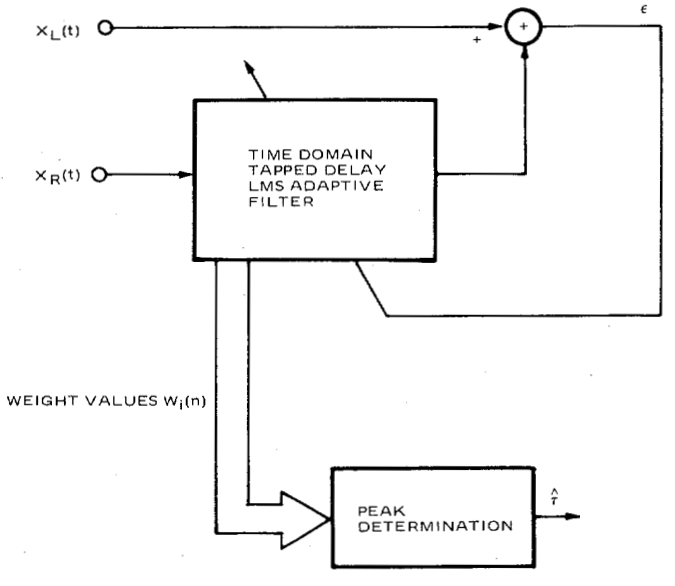
\includegraphics[width=0.5\textwidth]{figures/LMS.png}
	\end{center}
	\caption{TDE using an LMS filter}
	\label{fig:LMS}
\end{figure}


\subsection{Adaptive Eigenvalue Decomposition}
Adaptive eigenvalue decomposition (AED) algorithm was proposed to deal with TDE in reverberant environments. Unlike the crosscorrelation stated above, this algorithm first identifies the channel impulse responses from the source to the two sensors. The delay estimate is then determined by finding the direct paths from the two measured impulse responses. To do that, we observe that
  $$x_2[k] * g_1 = s[k] * g_2 * g_1 = x_1[k] * g_2$$
  
  Then, we can state that $R_u = 0$. This implies that vector $u$ which consists of two impulse responses is in the null space of R. More specifically, $u$ is the eigenvector of $R$ corresponding to the eigenvalue 0 ($u[k]=g_2[k] - g_1[k]$). We observe that $u$ can be uniquely determined if the following two conditions hold \cite{overview, aed}:
\begin{itemize}
  \item $g_1$ and $g_2$ do not share any common zeros.
  \item The covariance matrix $R$ is full rank.
\end{itemize}

  In case of noise, the covariance matrix will regularize. That will provoke that the algorithm stated above become inoperable because the lack of a 0 eigenvalue. To solve that we have implement this adaptive algorithm that calculate the eigenvector with minimum eigenvalue:
 $$u[k+1] = \frac{u[k] - \mu e[k] x[k]}{\text{norm}(u[k])}$$   where $\mu$ is the positive adaptation step.
 

  With the identified impulse responses $g_1$ and $g_2$, the time delay estimate is determined as the difference between two direct paths. That is $T_{\text{AED}} = \arg\max_T |g_2|-|g_1|$. 

  Finally, the noise will not be a problem with the time delay estimation because we only want to find the two direct path and not the whole impulse response. Then, AED is the best of the stated algorithms in front of noise and reverberation. 
